\input{../YKY-preamble.tex}

\usepackage[backend=biber]{biblatex}
\bibliography{../AGI-book}

\usepackage[CJKspace]{xeCJK}
\setCJKmainfont[BoldFont=SimHei,ItalicFont=KaiTi]{SimHei}

\title{《香港中立派宣言》\\{\footnotesize\color{red}[draft, \today]} }
\author{HK.neutrality@gmail.com}
\date{}

\setcounter{secnumdepth}{0}		% no section numbers
\renewcommand{\familydefault}{\sfdefault}

\begin{document}
\maketitle
\Large

\section{去除民主选举制}

\begin{itemize}
	\item 民主 令社会不断 回归到平均值,民主 不适合 人口多、发展中的国家,选举 is a waste of time

	\item {\color{red}[rephrase]} 民主是西方欺压其他民族的手段

	\item 西方历史上,民主的发源地 希腊雅典,亦没有因为有民主而免於战败。 民主的 Athens 被 Sparta 打败,即著名的 Pelopponesian War

	\item 柏拉图、亚里士多德 等哲学家 提出 政治的 \textbf{循环} (cycle): \\
		mob rule $\Rightarrow$ monarchy $\Rightarrow$ tyranny $\Rightarrow$ aristocracy $\Rightarrow$ oligarchy $\Rightarrow$ democracy $\Rightarrow$ mob rule 

	\item 「中国模式」令中国近10-20年经济起飞,必然做对了某些事。 其实 这证明了民主对於经济进步是不必要的。 印度有民主,但经济一样起唔到飞
	
	\item 中国在不平等条约下割让香港,所以中国没有义务 honor 中英联合声明,特别是 普选制度。 但在精神上香港中立派 传承了一国两制的安定繁荣 目标
	
\end{itemize}

\section{经济自由化 \textbullet 去除家长式管治}

\begin{itemize}
	\item 只有自由市场、经济竞争,才能令 社会进步
	\item 香港要放弃「家长式」管治 (paternalistic governance),政府要「放手」(\textbf{deregulation}) 让人们 自己 解决问题
	\item 亚洲 流行 家长式 管治,原因是 很多亚洲人像 \textbf{巨婴}。 左倾 和 民主 贪得无厌的诉求,都是基於 不劳而获的心态
	\item 美好的生活 $\supseteq$ 有赚钱的自由; 美国梦 (American dream) 指的是 美国人不论出身,都有可能透过努力成为富人
	\item Deregulation 的做法可以是: 企业联合集资,去除政府管制,并在过渡期获得制度上补偿
	\item 在香港进行 \textbf{土地改革} 不是没有可能的,但土地的经济学和一般财产可能有不同 \cite{Ryan-Collins2017} \cite{Farvacque-Vitkoviac1992} \cite{Blomley2004} \cite{Linklater2013} \cite{Adams2015},而且涉及「地产霸权」的利益
\end{itemize}

\section{全球化 \textbullet 香港中立}

\begin{itemize}
	\item 冷战后香港回归中国,但中国内战造成南北分裂局面,香港变成冷战后政治上的奇异点 (\textbf{singularity})
	\item 香港中立的优点可以吸引世界上 支持 种族平等 的人材 来港,而不是 吸引一班 racist「鬼佬」来港 坐享特权
	\item 亚洲人 的幼稚化,原因之一是 科技上无法追上欧美,导致强烈的出卖同胞欲望(宁愿做狗不做人)
	\item 唯有在国际上消除种族歧视,亚洲人才有希望过有尊严的生活
\end{itemize}

\section{土地/房屋 问题}

\begin{equation}
\vcenter{\hbox{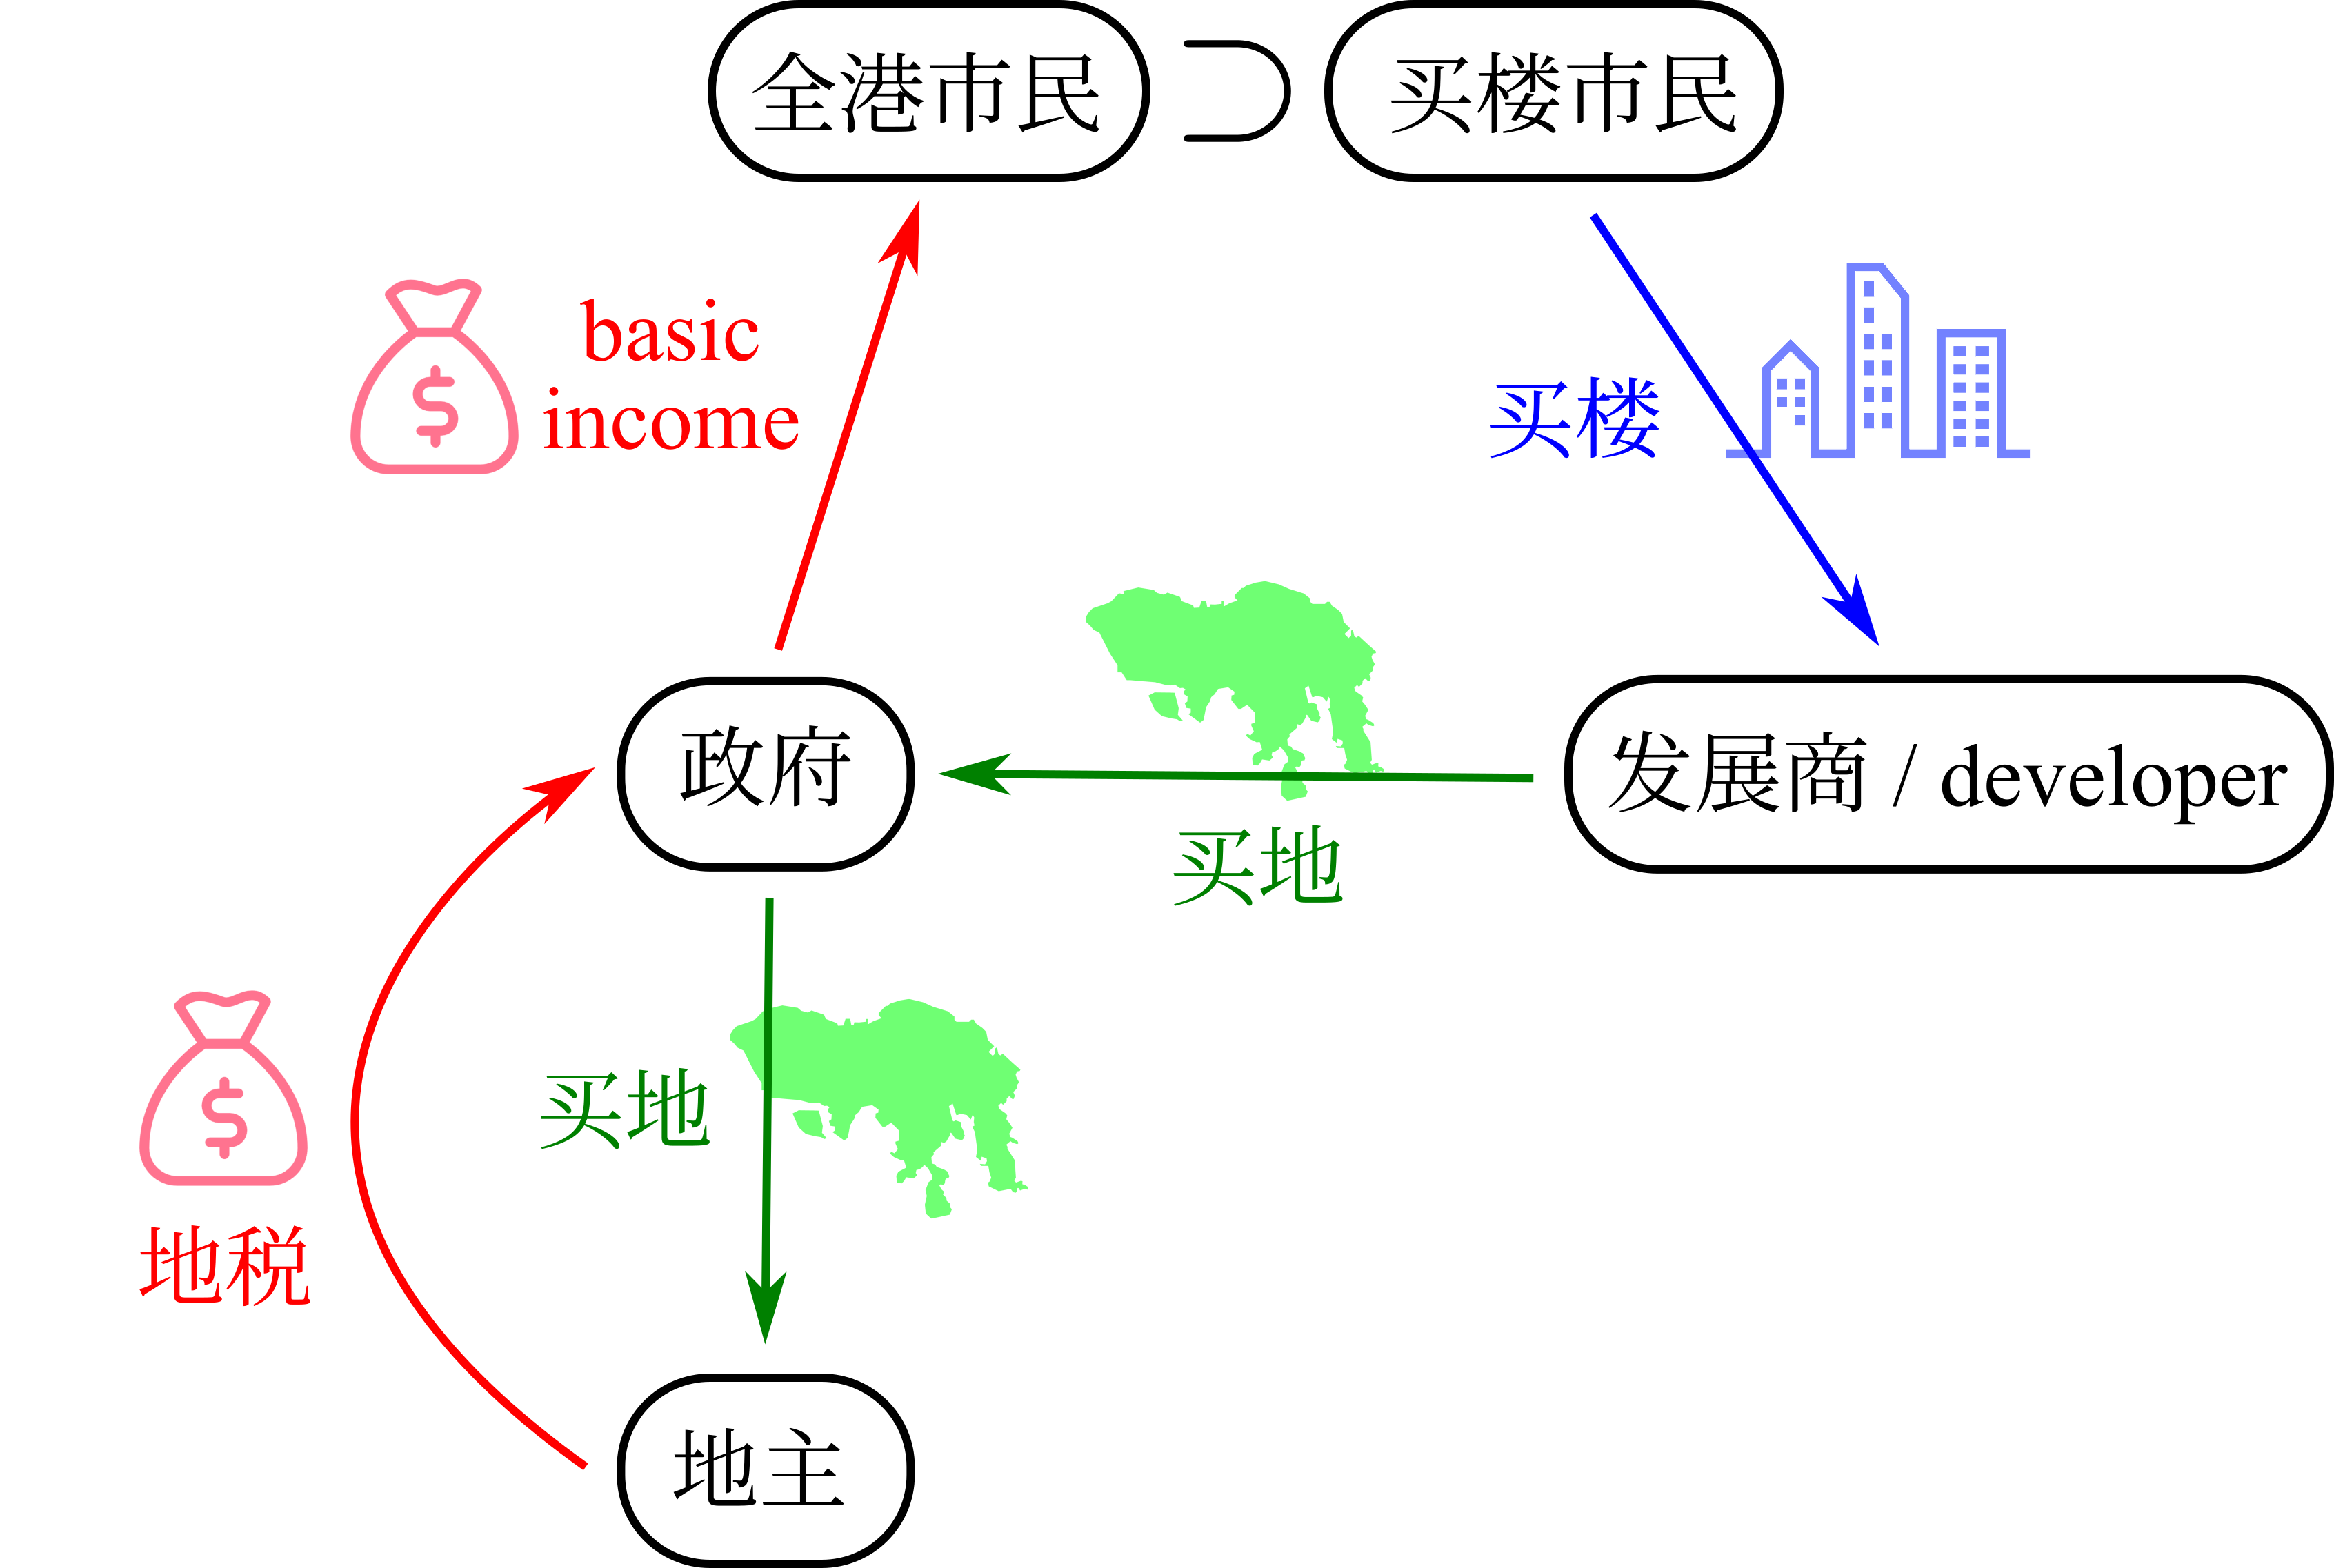
\includegraphics[scale=0.7]{housing-solution.png}}}
\end{equation}

问题: 如果 land tax 仍然不能降低楼价? 

增加 basic income 的理据

Rent-seeking 不是 land tax 的理由,但稀缺资源是

如是者,则 land tax 的目的,必然是将稀缺资源作公平分配

问题是 land tax 要收到什么程度?  也许,直到 平均收入 追得上为止。

但地税 会 transfer 给租户和住户,导致 楼价 仍然高企。  这样则进一步 增加 basic income.



\printbibliography

\end{document}